\section{Robustness of Dirichlet-based uncertainty models}
\label{sec:attack_dirichlet_model_008}

We analyze robustness of DBU models on tasks in connection with uncertainty estimation w.r.t.\ the following four aspects: \emph{accuracy}, \emph{confidence calibration}, \emph{label attack detection} and \emph{OOD detection}. Uncertainty is quantified by differential entropy, mutual information or pseudo counts. 
A formal definition of all uncertainty estimation measures is provided in the appendix (see Section~\ref{subsec:appendix_measurecomp}).  

Robustness of Dirichlet-based uncertainty models is evaluated based on \emph{label attacks} and a newly proposed type of attacks called \emph{uncertainty attacks}. 
While label attacks aim at changing the predicted class, uncertainty attacks aim at changing the uncertainty assigned to a prediction. 
All previous works are based on label attacks and focus on robustness w.r.t. the class prediction. Thus, we are the first to propose attacks targeting uncertainty estimates such as differential entropy and analyze desirable robustness properties of DBU models beyond the class prediction. 
Label attacks and uncertainty attacks both compute a perturbed input $\tilde{\x}\dataix$ close to the original input~$\x\dataix$ i.e. $|| \x\dataix - \tilde{\x}\dataix ||_2 < r$ where $r$ is the attack radius. This perturbed input is obtained by optimizing a loss function $l(\x)$ using Fast Gradient Sign Method (FGSM) or Projected Gradient Descent (PGD). Furthermore, we include a black box attack setting (Noise) which generates 10 noise samples from a Gaussian distribution, which is centered at the original input. From these 10 perturbed samples we choose the one with the greatest effect on the loss function and use it as attack. 
To complement attacks, we compute certificates on uncertainty estimates using median smoothing \cite{median_smoothing}. 


%Reviewer: avoid redundancy within assessment metric paragraphs, explain high level + differences
The following questions we address by our experiments have a common assessment metric and can be treated as binary classification problems: distinguishing between correctly and wrongly classified samples, discriminating between non-attacked input and attacked inputs or differentiating between ID data and OOD data. To quantify the performance of the models on these binary classification problems, we compute the area under the precision recall curve (AUC-PR).

Experiments are performed on two image data sets (MNIST \citep{mnist} and CIFAR10 \citep{cifar10}), which contain bounded inputs and two tabular data sets (Segment \citep{uci_datasets} and Sensorless drive \citep{uci_datasets}), consisting of unbounded inputs. Note that unbounded inputs are challenging since it is impossible to describe the infinitely large OOD distribution. As PriorNet requires OOD training data, we use two further image data sets (FashionMNIST \citep{fashionmnist} and CIFAR100 \citep{cifar10}) for training on MNIST and CIFAR10, respectively. All other models are trained without OOD data. To obtain OOD data for the tabular data sets, we remove classes from the ID data set (class window for the Segment data set and class 9 for Sensorless drive) and use them as the OOD data. Further details on the experimental setup are provided in the appendix (see Section~\ref{subsec:exp_setup}).



 


\subsection{Uncertainty estimation under label attacks}
\label{subsec:label_attacks}
%
Label attacks aim at changing the predicted class. To obtain a perturbed input with a different label, we maximize the cross-entropy loss $\tilde{\x}\dataix \approx \arg\max_{\x} l(\x) = \text{CE}(\vp\dataix, \vy\dataix)$ under the radius constraint. For the sake of completeness we additionally analyze label attacks w.r.t. to their performance of changing the class prediction and the accuracy of the neural network under label attacks constraint by different radii (see Appendix, Table~\ref{tab:acc_label_attack}). As expected and partially shown by previous works, none of the DBU models is robust against label attacks. %, neither on the image data sets nor on the tabular data sets.
However, we note that \PriorNet is slightly more robust than the other DBU models. This might be explained by the use of OOD data during training, which can be seen as some kind of robust training. 
%
From now on, we switch to the core focus of this work and analyze robustness properties of uncertainty estimation. 




\begin{table*}[ht]
	\centering
	%\begin{small}
	\resizebox{0.8\textwidth}{!}{
		\begin{tabular}{@{}rrrrrrrc|crrrrrr@{}}
			\toprule
			& \multicolumn{6}{c}{CIFAR10} & & & \multicolumn{6}{c}{Sensorless} \\
			\cmidrule{2-7}  \cmidrule{10-15}
			Att. Rad. & 0.0 & 0.1 & 0.2 & 0.5 & 1.0 & 2.0 & & & 0.0 & 0.1 & 0.2 & 0.5 & 1.0 & 2.0  \\
			\midrule
			%& \multicolumn{7}{c}{MNIST} & & & \multicolumn{7}{c}{CIFAR10} \\
			\PostNetacro{}  &  \bf{98.7} &  88.6 &  56.2 &   7.8 &   1.2 &   0.4 &  & %0.3 & & 
			&  99.7 &   8.3 &   3.9 &  3.6 &  \bf{7.0} &  \bf{9.8} \\%&  \bf{11.3} \\
			\PriorNet &  92.9 &  77.7 &  60.5 &  \bf{37.6} &  \bf{24.9} &  \bf{11.3} &  & %\bf{3.0} & & 
			&  99.8 &  10.5 &   3.2 &  0.7 &  0.2 &  0.2 \\%&   2.2 \\ 
			\DDNet    &  97.6 &  \bf{91.8} &  \bf{78.3} &  18.1 &   0.8 &   0.0 &  &%0.0 & &
			&  99.7 &  11.9 &   1.6 &  0.4 &  0.2 &  0.1 \\%&   0.2 \\ 
			\EvNet    &  97.9 &  85.9 &  57.2 &  10.2 &   4.0 &   2.4 &  &%0.3 & & 
			&  \bf{99.9} &  \bf{22.9} &  \bf{13.0} &  \bf{6.0} &  3.7 &  3.2 \\%&   3.1 \\
			\bottomrule
		\end{tabular}}
	%\end{small}
	\caption{Distinguishing between correctly predicted and wrongly predicted labels based on the differential entropy under PGD label attacks (metric: AUC-PR).}
	\label{tab:conf_label_attack}
\end{table*}







\begin{center}
	\textbf{Is low uncertainty a reliable indicator of correct predictions?}
\end{center}
\underline{\emph{Expected behavior:}}  Predictions with low uncertainty are more likely to be correct than high uncertainty predictions. 
\underline{\emph{Assessment metric:}} We distinguish between correctly classified samples (label 0) and wrongly classified ones (label 1) based on the differential entropy scores produced by the DBU models \citep{malini2018}. Correctly classified samples are expected to have low differential entropy, reflecting the model's confidence, and analogously wrongly predicted samples are expected to have higher differential entropy. 
%\dz{State that the metric is AUC-PR?} 
\underline{\emph{Observed behavior:}} Note that the positive and negative class are not balanced, thus, the use of AUC-PR scores \citep{imbalance_apr} are important to enable meaningful measures. While uncertainty estimates are indeed an indicator of correctly classified samples on unperturbed data, none of the models maintains its high performance on perturbed data computed by PGD, FGSM or Noise label attacks (see. Table~\ref{tab:conf_label_attack}, \ref{tab:conf_label_attack_fgsm} and \ref{tab:conf_label_attack_noise_attack}). Thus, using uncertainty estimates as indicator for correctly labeled inputs is not robust to adversarial perturbations. This result is notable, since the used attacks do not target uncertainty. 





\vspace{1em}
\begin{table*}[ht]
	\centering
	%\begin{small}
	\resizebox{0.8\textwidth}{!}{
		\begin{tabular}{@{}rrrrrrc|crrrrr@{}}
			\toprule
			& \multicolumn{5}{c}{CIFAR10} & & & \multicolumn{5}{c}{Sensorless} \\
			\cmidrule{2-6}  \cmidrule{9-13}
			Att. Rad. & 0.1 & 0.2 & 0.5 & 1.0 & 2.0 & & & 0.1 & 0.2 & 0.5 & 1.0 & 2.0 \\
			\midrule
			\PostNetacro{}  &  \bf{63.4} &  \bf{66.9} &  42.1 &  32.9 &  31.6 &  &%31.2 & & 
			&  47.7 &  42.3 &  36.9 &  \bf{48.5} &  \bf{85.0} \\%&  \bf{99.0} \\ 
			\PriorNet &  53.3 &  56.0 &  55.6 &  \bf{49.2} &  42.2 & &%  35.4 & & 
			&  38.8 &  33.6 &  31.4 &  33.1 &  40.9 \\%&  53.5 \\ 
			\DDNet    &  55.8 &  60.5 &  \bf{57.3} &  38.7 &  32.3 & &% 31.4 & & 
			&  \bf{53.5} &  42.2 &  35.0 &  32.8 &  32.6 \\%&  33.9 \\ 
			\EvNet    &  48.4 &  46.9 &  46.3 &  46.3 &  \bf{44.5} & &% \bf{42.5} & &
			&  48.2 &  \bf{42.6} &  \bf{38.2} &  36.0 &  37.2 \\%&  41.7 \\
			\bottomrule 			
		\end{tabular}}
	%\end{small}
	\caption{Label Attack-Detection by normally trained DBU models based on differential entropy under PGD label attacks (AUC-PR).}
	\label{tab:label_attack_detect}
\end{table*}








%\vspace{-0.5em}
\begin{center}
	\textbf{Can uncertainty estimates be used to detect label attacks against the class prediction?}	
\end{center}
\underline{\emph{Expected behavior:}} Adversarial examples are not from the natural data distribution. Therefore, DBU models are expected to detect them as OOD data by assigning them a higher uncertainty. We expect that perturbations computed based on a bigger attack radius~$r$ are easier to detect as their distance from the data distribution is larger. 
\underline{\emph{Assessment metric:}} The goal of attack-detection is to distinguish between unperturbed samples (label 0) and perturbed samples (label 1). Uncertainty on samples is quantified by the differential uncertainty \citep{malini2018}. Unperturbed samples are expected to have low differential entropy, because they are from the same distribution as the training data, while perturbed samples are expected to have a high differential entropy. 
%Further results based on other uncertainty measures are provided in the appendix. 
\underline{\emph{Observed behavior:}} Table~\ref{tab:acc_label_attack} shows that the accuracy of all models decreases significantly under PGD label attacks, but none of the models is able to provide an equivalently increasing attack detection rate (see Table~\ref{tab:label_attack_detect}). Even larger perturbations are hard to detect for DBU models. 

Similar results are obtained when we use mutual information or the precision~$\alpha_0$ to quantify uncertainty (see appendix Table~\ref{tab:conf_label_attack_mi} and~\ref{tab:conf_label_attack_alpha}).
Although PGD label attacks do not explicitly consider uncertainty, they seem to generate adversarial examples with similar uncertainty as the original input. 
Such high-certainty adversarial examples are illustrated in Figure~\ref{fig:attaked_samples_labels}, where certainty is visualized based on the precision~$\alpha_0$, which is supposed to be high for ID data and low for OOD data. While the original input (perturbation size $0.0$) is correctly classified as frog and ID data, there exist adversarial examples that are classified as deer or bird. The certainty ($\alpha_0$-score) on the prediction of these adversarial examples has a similar or even higher value than on the prediction of the original input. Using the differential entropy to distinguish between ID and OOD data results in the same ID/OOD assignment since the differential entropy of the three right-most adversarial examples is similar or even smaller than on the unperturbed input. 







Under the less powerful FGSM and Noise attacks (see Appendix), DBU models achieve mostly higher attack detection rates than under PGD attacks. This suggests that uncertainty estimation is able to detect weak attacks, which is consistent with the observations in \citep{malinin2018_adetect} but fails under stronger PGD attacks. 
%
\begin{figure}[ht]
	\centering
	\resizebox{0.42\textwidth}{!}{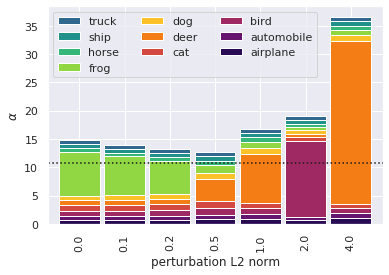
\includegraphics[width=\textwidth]{sections/008_icml2021/eval/ddnet_label_id_cifar10_alphas.png}}%
	\resizebox{0.42\textwidth}{!}{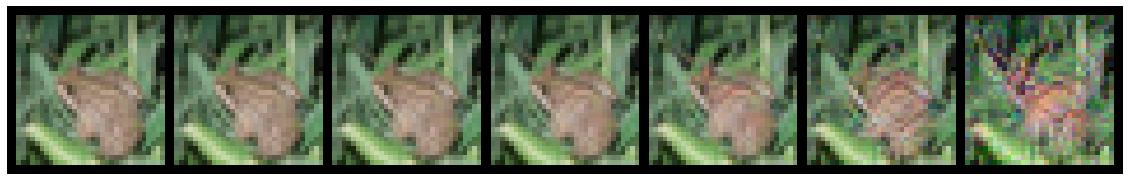
\includegraphics[width=\textwidth]{sections/008_icml2021/eval/ddnet_label_id_cifar10_images.png}}
	\caption{Input and predicted Dirichlet-parameters under label attacks (dotted line: threshold to distinguish ID and OOD data). % based on the precision~$\alpha_0$.
		%-14.2216765174
		%0.0 [-17.875761]
		%0.1 [-17.257824]
		%0.2 [-16.648003]
		%0.5 [-15.014889]
		%1.0 [-17.504786]
		%2.0 [-22.63896]
		%4.0 [-24.941536]
	}
	\label{fig:attaked_samples_labels}
\end{figure}


On tabular data sets, \PostNetacro{} shows a better label attack detection rate for large perturbations. This observation might be explained by the fact that the density estimation of the ID samples has been shown to work better for tabular data sets \citep{charpentier2020}. 
%
Overall, none of the DBU models provides a reliable indicator for adversarial inputs that target the class prediction. 





\vspace{.4mm}
\begin{table*}[ht]
	\centering
%	\begin{small}
	\resizebox{\textwidth}{!}{
		\begin{tabular}{@{}rrrrrrrc|crrrrrr@{}}
			\toprule
			& \multicolumn{6}{c}{ID-Attack (non-attacked OOD)} &  & &  \multicolumn{6}{c}{OOD-Attack (non-attacked ID)} \\
			\cmidrule{2-7}  \cmidrule{10-15}
			Att. Rad. & 0.0 & 0.1 & 0.2 & 0.5 & 1.0 & 2.0 & & &
			0.0 & 0.1 & 0.2 & 0.5 & 1.0 & 2.0  \\
			\midrule
			& \multicolumn{14}{c}{\textbf{CIFAR10 -- SVHN}} \\
			\PostNetacro{}  &  81.8 &  64.3 &  47.2 &  22.4 &  17.6 &  \bf{16.9} &  &%\bf{16.4} & &
			&  81.8 &  60.5 &  40.7 &  23.3 &  21.8 &  19.8 \\%&  18.1 \\ 
			\PriorNet &  54.4 &  40.1 &  30.0 &  17.9 &  15.6 &  15.4 &  &%15.4 & &
			&  54.4 &  40.7 &  30.7 &  19.5 &  16.5 &  15.7 \\%&  15.4 \\
			\DDNet    &  \bf{82.8} &  \bf{71.4} &  \bf{59.2} &  \bf{28.9} &  16.0 &  15.4 & &% 15.4 & &
			&  \bf{82.8} &  \bf{72.0} &  \bf{57.2} &  20.8 &  15.6 &  15.4 \\%&  15.4 \\
			\EvNet    &  80.3 &  62.4 &  45.4 &  21.7 &  \bf{17.9} &  16.5 &  &%15.6 & &
			&  80.3 &  58.2 &  46.5 &  \bf{34.6} &  \bf{28.0} &  \bf{23.9} \\%&  \bf{21.0} \\
			\midrule
			& \multicolumn{14}{c}{\textbf{Sens. -- Sens. class 10, 11}} \\
			\PostNetacro{}  &  \bf{74.5} &  \bf{39.8} &  \bf{36.1} &  \bf{36.0} &  \bf{45.9} &  \bf{46.0} & &% \bf{46.0} & &
			&  \bf{74.5} &  \bf{43.3} &  \bf{42.0} &  \bf{32.1} &  \bf{35.1} &  \bf{82.6} \\%&  \bf{99.4} \\
			\PriorNet &  32.3 &  26.6 &  26.5 &  26.5 &  26.6 &  28.3 & &% 38.6 & &
			&  32.3 &  26.7 &  26.6 &  26.6 &  27.0 &  30.4 \\%&  36.8 \\ 
			\DDNet    &  31.7 &  26.8 &  26.6 &  26.5 &  26.6 &  27.1 & &% 30.5 & &
			&  31.7 &  27.1 &  26.7 &  26.7 &  26.8 &  26.9 \\%&  27.3 \\ 
			\EvNet    &  66.5 &  30.5 &  28.2 &  27.1 &  28.1 &  31.8 & &% 37.5 & &
			&  66.5 &  38.7 &  36.1 &  30.2 &  28.2 &  28.8 \\%&  32.2 \\
			\bottomrule
		\end{tabular}}
%	\end{small}
	\caption{OOD detection based on differential entropy under PGD uncertainty attacks against differential entropy computed on ID data and OOD data (metric: AUC-PR).}
	\label{tab:id_ood_attacks}
\end{table*}









\subsection{Attacking uncertainty estimation}
\label{subsec:uncertainty_attacks}

DBU models are designed to provide sophisticated uncertainty estimates (beyond softmax scores) alongside predictions and use them to detect OOD samples. In this section, we propose and analyze a new attack type that targets these uncertainty estimates. 
DBU models enable us to compute uncertainty measures i.e. differential entropy, mutual information and precision~$\alpha_0$ in closed from (see \citep{malini2018} for a derivation). Uncertainty attacks use this closed form solution as loss function for PGD, FGSM or Noise attacks. 
Since differential entropy is the most widely used metric for ID-OOD-differentiation, we present results based on the differential entropy loss function $\tilde{\x}\dataix \approx \arg\max_{\x} l(\x) = \text{Diff-E}(\text{Dir}(\mathbf{\alpha}\dataix))$: 
%
\begin{equation}
\begin{aligned}
	\text{Diff-E}(\text{Dir}(\mathbf{\alpha}\dataix))  = &\sum_c^K \ln \Gamma (\alpha_c^{(i)}) - \ln \Gamma (\alpha_0^{(i)}) \\
	&- \sum_c^K (\alpha_c^{(i)} -1) \cdot (\Psi (\alpha_c^{(i)}) - \Psi (\alpha_0^{(i)}))
\end{aligned}
\end{equation}
%
where $\alpha_0^{(i)} = \sum_c \alpha_c^{(i)}$. 
Result based on further uncertainty measures, loss functions and more details on attacks are provided in the appendix. 


We analyze the performance of DBU models under uncertainty attacks w.r.t.\ two tasks. First, uncertainty attacks are computed on ID data aiming to indicate it as OOD data, while OOD data is left non-attacked. Second, we attack OOD data aiming to indicate it as ID data, while ID data is not attacked. Hence, uncertainty attacks target at posing ID data as OOD data and vice versa.


\begin{figure}[ht!]
    \centering
        \begin{subfigure}[t]{0.49\columnwidth}
        \centering
        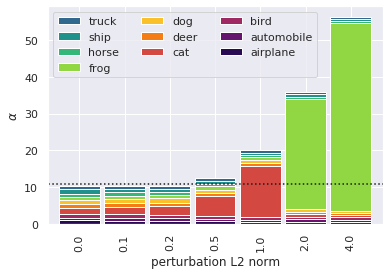
\includegraphics[width=0.99 \textwidth]{sections/008_icml2021/eval/ddnet_unc_ood_cifar10_alphas.png}
    \end{subfigure}%
    \begin{subfigure}[t]{0.49\columnwidth}
        \centering
        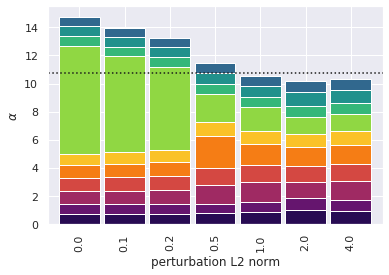
\includegraphics[width=0.99 \textwidth]{sections/008_icml2021/eval/ddnet_unc_id_cifar10_alphas.png}
    \end{subfigure}%


    \begin{subfigure}[t]{0.49 \columnwidth}
        \centering
        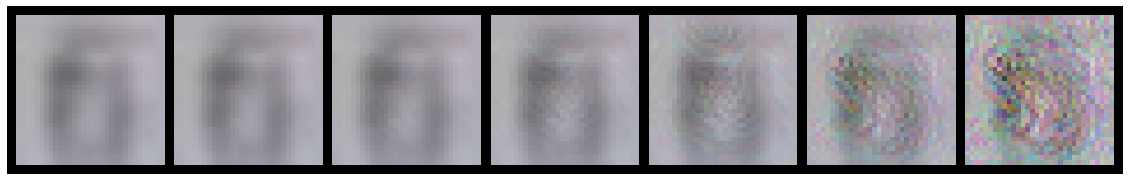
\includegraphics[width=0.99 \textwidth]{sections/008_icml2021/eval/ddnet_unc_ood_cifar10_images.png}
        \caption{OOD uncertainty attack
        %-14.2216765174
        %0.0 [-13.115507]
        %0.1 [-13.353642]
        %0.2 [-13.723262]
        %0.5 [-16.341246]
        %1.0 [-22.298155]
        %2.0 [-28.071136]
        %4.0 [-33.148224]
        }
        \label{fig:attaked_samples_idood_a}
    \end{subfigure}%
        \begin{subfigure}[t]{0.49 \columnwidth}
        \centering
        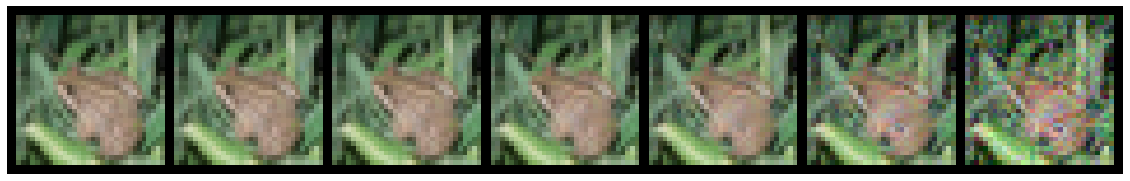
\includegraphics[width=0.99 \textwidth]{sections/008_icml2021/eval/ddnet_unc_id_cifar10_images.png}
        \caption{ID uncertainty attack
        %-14.2216765174
        %0.0 [-17.875761]
        %0.1 [-17.256058]
        %0.2 [-16.65203]
        %0.5 [-14.321844]
        %1.0 [-13.6354265]
        %2.0 [-13.046129]
        %4.0 [-13.1426115]
        }
        \label{fig:attaked_samples_idood_b}
    \end{subfigure}%
    \caption{ID and OOD input with corresponding Dirichlet-parameters under uncertainty attacks (dotted line: threshold to distinguish ID and OOD).}
    \label{fig:attaked_samples_idood}
	%\vspace{-.5cm}
\end{figure}




\begin{center}
	\textbf{Are uncertainty estimates a robust feature for OOD detection?}	
\end{center}
\underline{\emph{Expected behavior:}} We expect DBU models to be able to distinguish between ID and OOD data by providing reliable uncertainty estimates, even under small perturbations. Thus, we expect uncertainty estimates of DBU models to be robust under attacks. 
%
\underline{\emph{Assessment metric:}} We distinguish between ID data (label 0) and OOD data (label 1) based on the differential entropy as uncertainty scoring function \citep{malini2018}. Differential entropy is expected to be small on ID samples and high on OOD samples. Experiments on further uncertainty measure and results on the AUROC metric are provided in the appendix. 
%
\underline{\emph{Observed behavior:}} OOD samples are perturbed as illustrated in  Figure~\ref{fig:attaked_samples_idood}. Part (a) of the figure illustrates an OOD-samples, that is correctly identified as OOD. Adding adversarial perturbations $\geq 0.5$ changes the Dirichlet parameters such that the resulting images are identified as ID, based on precision or differential entropy as uncertainty measure. Perturbing an ID sample (part (b)) results in images that are marked as OOD samples. 
OOD detection performance of all DBU models rapidly decreases with the size of the perturbation, regardless of whether attacks are computed on ID or OOD data (see Table~\ref{tab:id_ood_attacks}). This performance decrease is also observed with AUROC as metric, attacks based on FGSM, Noise, when we use mutual information or precision~$\alpha_0$ to distinguish between ID samples and OOD samples (see appendix Table~\ref{tab:id_ood_attacks_part2} - \ref{tab:id_ood_attacks_measure_diffE_aupr_noise}). 
Thus, using uncertainty estimation to distinguish between ID and OOD data is not robust. 



